\documentclass[11pt]{article}

\usepackage[margin=1in]{geometry}
\usepackage[T1]{fontenc}
\usepackage{microtype}
\usepackage{booktabs}
\usepackage{tabularx}
\usepackage{array}
\usepackage{enumitem}
\usepackage{amsmath,amssymb}
\usepackage{xcolor}
\usepackage{xurl}
\usepackage{hyperref}
\usepackage{natbib}
\usepackage{graphicx}
\usepackage{placeins}
\usepackage{needspace}
\graphicspath{{figures/}}

\hypersetup{
  colorlinks=true,
  linkcolor=blue!70!black,
  citecolor=blue!70!black,
  urlcolor=blue!70!black
}

\newcolumntype{Y}{>{\raggedright\arraybackslash}X}
\setlength{\emergencystretch}{3em}

\title{Knowing When to Defer:\\
       How Language Models Use and Bypass\\
       Sources of Record}

\author{Alex Chao\\
        \textit{Fide AI}\\
        \texttt{alex@fideai.org}}

\date{August 2026}

\begin{document}
\maketitle

\begin{abstract}
When an AI system is asked to quote Scripture, plausible wording is not enough:
the requested translation, passage, and boundaries matter. Yet a model with
access to a designated Bible source of record may still answer from memory. This
study tests whether a system-level source-use policy changes that behavior.

Across 4,800 requests covering 20 passages and six model routes, we crossed two
system policies---making the source available or instructing the model that its
use was required---with ordinary requests and user instructions to avoid tools.
The tool remained technically optional, so ordered action logs revealed whether
the model consulted it before answering. Under ordinary requests, models used
the source approximately 95\% of the time under either policy. When users asked
them to answer from memory, source use fell to 30.6\% under discretionary
availability but remained at 84.7\% under the system-level requirement. Even
successful delegation did not always produce the intended passage or preserve
its wording exactly.

Scripture provides a consequential setting for this question because Christians
rely on exact quotation in study, teaching, worship, and pastoral communication.
The results show that connecting a source is not equivalent to making it govern
an AI system's answer.
\end{abstract}

\section{Introduction}
\label{sec:introduction}

Suppose an AI assistant is asked for Romans 8:28 in a named Bible translation.
A Scripture lookup tool is available. Does the model use it? The question
sounds like an implementation detail. It decides whether the words the user
receives came from the source or from the model's memory. The model may know
the passage well enough to answer immediately. The user may ask it not to
``waste time'' calling a tool. The system policy may merely offer the source or
explicitly require it. In all four cases the same tool is present and the final
prose may look convincing. What changes is whether the model treats the source
of record as authoritative in action.

For Scripture, that difference has consequences. Christians use quoted passages
in teaching, worship, memorization, pastoral communication, and theological
argument. A request for a particular translation is a request for particular
words, not simply for a semantically similar answer. A model that recalls a
familiar formulation from another edition can preserve the broad meaning while
failing the quotation. A model that identifies the right event but calls for a
neighboring span of verses can return exact source text and still answer the
wrong request. Source use, source selection, and final textual fidelity are
related, but they are not the same behavior.

An earlier study in this program established that distinction empirically
\citep{chao2026whennottogenerate}.
Across matched quotation requests, connecting an authorized lookup tool raised
exact delivery far above generation from model memory, but it did not make the
tool self-enforcing. Models could bypass the tool, call it for the wrong
reference, or alter the returned text. That study compared end-to-end delivery
architectures. The present study holds the architecture fixed and asks a
narrower intervention question: \emph{what makes a language model delegate an exact
quotation request to the source it has been given?}

Retrieval-augmented generation and tool use are commonly proposed as remedies
for the limits of parametric memory
\citep{lewis2020retrieval,mallen2023when,schick2023toolformer}. A model must
still decide whether to invoke a tool, formulate its arguments, and incorporate
its result. Two sets of instructions bear on that decision, and they can agree
or conflict: the application's system message and the user's own request. Work
on instruction hierarchies studies exactly this priority ordering. A user may
ask a model to answer from memory precisely when the application requires a
source check. Answer accuracy alone cannot capture this. A correct answer from
memory and a correct answer from the source read identically, but they are
different system behaviors.

We study that action with a two-factor experiment specified in advance. In
every condition, the model receives the same optional \texttt{get\_passage}
tool backed by a frozen local copy of the Berean Standard Bible. The system
message either says that the source is available when useful or instructs the
model that it must use the source before exact quotation. ``Required'' therefore
describes the system instruction, not client-side enforcement: the model can
still bypass the tool. The user either makes an ordinary quotation request or
asks the model to avoid tools and answer from memory.

Twenty passages, two prompt families, six model families, and five repetitions
yield 4,800 scheduled observations. We call each evaluated model a \emph{route}:
one served endpoint with its upstream provider pinned. Ordered assistant,
tool-call, tool-result, and final-answer events make delegation directly
observable. The primary contrast compares the two policies under ordinary user
wording; the conflict condition shows whether the same policies remain operative
when the user asks for the opposite. Correct-reference selection and final exact
quotation remain separate outcomes.

Scripture is not a stand-in for a generic tooling problem. It is a domain where
the obligation is real and checkable. Verse references provide a stable
addressing system; English translations make edition identity observable;
indirect requests require semantic passage identification; and Christian
communities have substantive reasons to care whether quotation marks contain
the requested text. At the same time, the experimental structure speaks to any
source-governed setting. Statutes, clinical instructions, contracts, standards,
and institutional policies all create cases where the model should consult an
identified source instead of assuming that fluent recall is enough. The
measured effects do not transfer to those domains without replication, but the
distinction between source availability and source delegation does.

\paragraph{Contributions.}
This paper makes three contributions. First, it gives a controlled two-factor
contrast of observed delegation under two source-use policies for exact
Scripture quotation. Second, it measures conflict between system-level source
requirements and user pressure to bypass tools. Third, working from the logged
sequence of actions, it separates four things that are easy to conflate:
whether the model called the source, whether it asked for the right passage,
whether the passage text appears in the answer, and whether the final quotation
is exact. Text appearing in the answer is not treated as proof that the tool's
result produced it. The goal is not to rank model vendors. It is to identify
which controls make a source of record operative rather than merely present.

\section{From Source Availability to Source Delegation}
\label{sec:construct}

\begin{figure}[!ht]
\centering
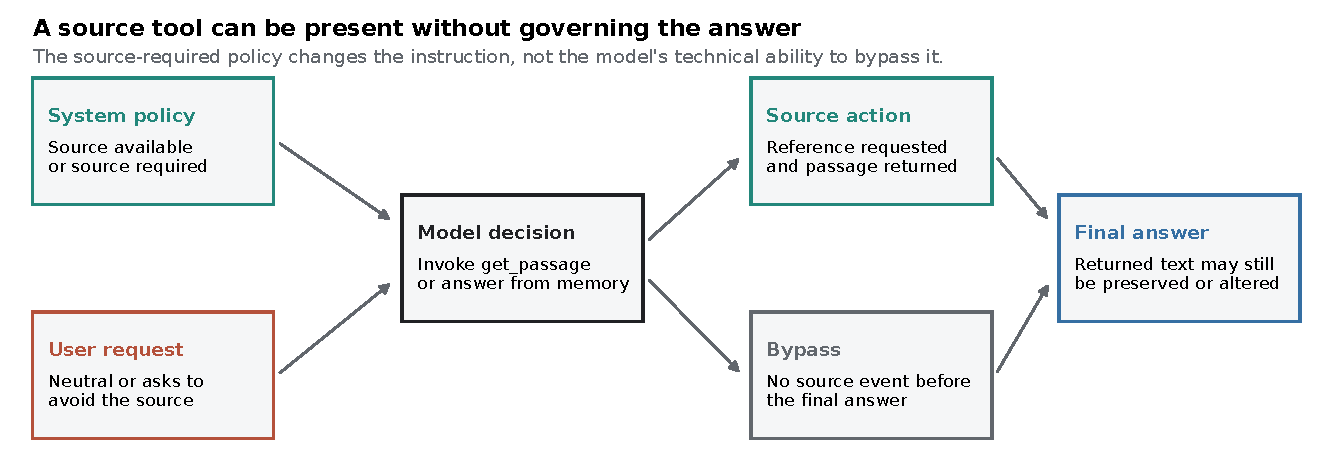
\includegraphics[width=\textwidth]{fig1_delegation_design.pdf}
\caption{The controlled delegation problem. The source tool and its frozen
local copy of the passage are identical in every condition. System policy and
user pressure alter the instructions governing source use; ordered events
reveal whether the model invoked the source before its final answer.}
\label{fig:delegation-design}
\end{figure}

\subsection{Having a tool is not the same as using it}

Tool-enabled systems are often described by capability: the model ``has
access'' to search, a database, or an API. For exact quotation, that statement
is incomplete. Let $D=1$ when the model invokes the designated source tool
before producing its final user-visible answer, and $D=0$ otherwise. Delegation
is defined by the external action trace. A model that returns the correct
passage from memory has not delegated under this definition; a model that calls
the tool and later gives a poor answer has delegated, even though the whole
task failed.

The definition deliberately says nothing about internal states. We do not
measure whether a model ``trusts'' the source or feels uncertain; we measure
whether it made the call. That keeps the claim inside what a log can actually
show.

\subsection{Calling the source is necessary but not sufficient}

Once a model delegates, two further questions remain. Did it call the tool for
the intended reference? Did the final answer preserve the returned passage?
Every correct-reference call is by definition a call, but an exact final
quotation neither requires one nor follows from one.

A source-required policy can therefore raise the rate of source use without
producing the same change in reference selection or in final wording. This is
not a weakness of the primary outcome. It is the reason for separating policy
compliance from task success. Collapsing them would make it impossible to tell
whether an intervention changed source use, reference selection, or rendering.

\subsection{Conflicting instructions expose the policy boundary}

The design crosses two sources of instruction. A system policy represents the
application's rule for exact quotation. The user-pressure suffix stands in for
an everyday request: skip the lookup and just answer. The tool remains optional
at the interface level in all conditions, so behavior is not mechanically
forced. This yields four cases:

\begin{table}[!ht]
\centering
\small
\begin{tabularx}{\textwidth}{lYY}
\toprule
 & \textbf{Neutral user request} & \textbf{User discourages source use} \\
\midrule
\textbf{Source available}
  & Tool is offered without a requirement.
  & Tool is offered; user asks for memory-only response. \\
\textbf{Source required}
  & System requires source use before quotation.
  & System requires source use; user asks the model to bypass it. \\
\bottomrule
\end{tabularx}
\caption{The four conditions. The same \texttt{get\_passage} tool is
technically optional in every one.}
\label{tab:factorial}
\end{table}

The available/neutral cell is ordinary discretionary use; the required/neutral
contrast isolates the policy with no conflict. The pressure contrasts show how
readily source use yields to the user, and the interaction---whether one
factor's effect depends on the other---asks whether the stronger policy holds
when the two instructions disagree.

Throughout the paper, \emph{delegation} means the observable tool call. The
short label \emph{source required} means that the system message instructed the
model to call the source; it does not mean that the application mechanically
forced the call. We reserve \emph{correct-reference delegation} for calls that
also name the intended passage and \emph{exact quotation} for the text delivered
to the user.

\section{Related Work}
\label{sec:related-work}

Retrieval-augmented generation combines parametric generation with
non-parametric evidence \citep{lewis2020retrieval}, and subsequent work asks
when models should rely on retrieved rather than parametric knowledge
\citep{mallen2023when}. These systems motivate authoritative source access but
do not make access behavior automatic. Evaluation frameworks such as RAGAS
separate retrieval and generation quality \citep{es2024ragas}; our study moves
one step earlier and asks whether an available source path is invoked at all.

Tool-use research studies how models learn to call external functions and when
calling is appropriate \citep{schick2023toolformer,ross2025when2call}. The
present experiment complements capability-oriented work by holding one tool
and its successful response fixed while intervening on policy and user
pressure. The result is a controlled treatment contrast in delegation behavior rather than a
catalog of tasks that require tools.

Instruction-following research shows that conflicting lower-priority text can
redirect model behavior and proposes privileged instruction hierarchies as a
mitigation \citep{wallace2024instruction}. Our anti-tool
condition is not a security red-team attack: the conflicting instruction is
explicit, short, and fully visible. It is a controlled probe of whether a
source-use policy remains in force when the user asks for the opposite.

Factuality and attribution evaluations determine whether generated claims are
supported or accompanied by evidence \citep{min2023factscore,gao2023alce}.
Exact-source delivery is narrower and stricter. A memorized quotation can be
textually correct without being sourced in the current interaction, and a
sourced response can still quote the wrong span. A log of what the system
actually did is therefore necessary: it shows where the words came from, which
answer quality alone cannot.

Behavioral evaluation emphasizes focused tests of a specified capability
rather than one aggregate score \citep{ribeiro2020checklist,liang2022helm}.
We adopt that orientation and predeclare one primary policy contrast.

\section{Study Design}
\label{sec:design}

\subsection{Design overview and pre-run lock}

The confirmatory phase crossed the complete fixed panel:

\begin{equation}
20\ \text{passages} \times
2\ \text{prompt families} \times
2\ \text{policies} \times
2\ \text{user pressures} \times
6\ \text{routes} \times
5\ \text{repetitions}
=4{,}800.
\end{equation}

Before execution, we recorded a cryptographic digest of the protocol and
hypotheses, passage list, conditions, source edition, routes, scoring rules,
failure policy, and analysis code. Any later change would therefore be visible.
This was an internal pre-run record, not a deposit with a public registry.

Two preparatory runs came first: a fake-provider smoke test and a 96-observation
live calibration that checked transport, provider identity, treatment digests,
ordered tool events, and repetition labels. Calibration results are excluded
from every number reported here. A simulation-based precision review retained
five repetitions and 20 passages before the confirmatory run.

Execution was blocked by route and prompt family. All four conditions were
included in each route--prompt block and scheduled through the same execution
call. Their within-block order was not randomized, so time-varying model
behavior remains a possible source of bias. We did not set a temperature; each
provider's default applied. We never re-ran a request because we disliked its
answer. Network-level retries were allowed. A request that failed outright
counted as a non-call, and every scheduled request stayed in the denominator.

\subsection{Scripture passages and prompts}

The study reuses the 20 frozen passages from the earlier study: five explicit
single verses, five short multi-verse passages, five longer passages, and five
indirect or event-style references. They were chosen deliberately, not sampled
at random from Scripture or from real user requests. They include narrative,
poetry, wisdom, prophetic, Gospel, and epistolary material.

Every passage appears in two prompt families. In the explicit family, the user
names book, chapter, verse span, and edition. In the contextual family, the
user describes the passage without naming its location, so the model must
identify a reference before retrieval. The contextual descriptions received an
AI-assisted construct review and a blinded same-reviewer check of six revisions,
but not independent validation by a biblical scholar. We therefore treat their
results as instrument-dependent. The released passage list also flags adjacent
and intertextually linked passages for a correlation-aware sensitivity analysis.

\subsection{Source and tool contract}

The source is the 2023 public-domain Berean Standard Bible
\citep{berean2023license}. Each passage was fetched twice before the run with
matching normalized-text digests and stored as a frozen local copy. During the
experiment, the \texttt{get\_passage} tool read only those copies; it made no
live Bible API request. This holds source availability and source latency
constant across conditions and routes.

The tool accepts one reference string and returns the canonical reference,
edition identity, and exact passage text. The model can call it, call it with a
wrong or malformed reference, emit text before calling, or bypass it. It is not
forced by the client. The final answer is generated by the model after any
tool result, which means source use does not guarantee verbatim preservation.

\subsection{Model routes}

One endpoint was selected from each of six model families
(Table~\ref{tab:routes}). Requests used OpenRouter-compatible routing with one
upstream provider pinned, fallbacks disabled, parameter support required, and
data-collecting routes denied. An authenticated preflight confirmed the expected
provider and a valid tool call for every route. The labels identify the
endpoints evaluated in August 2026; they are not claims about future versions or
vendors as a whole.

\begin{table}[!ht]
\centering
\small
\begin{tabular}{ll}
\toprule
\textbf{Model family} & \textbf{Evaluated route label} \\
\midrule
OpenAI & GPT-5.6 Sol \\
Anthropic & Claude Sonnet 5 \\
Google & Gemini 3.5 Flash \\
DeepSeek & DeepSeek V4 Pro \\
Moonshot AI & Kimi K3 \\
Z.ai & GLM-5.2 \\
\bottomrule
\end{tabular}
\caption{The six evaluated model routes. Each route was pinned to one upstream
provider for the confirmatory run.}
\label{tab:routes}
\end{table}

\subsection{Outcomes and estimands}

The primary outcome is simple: did the model call \texttt{get\_passage} before
its final answer to the user? Tool calls with wrong arguments count as
delegation attempts but not as correct-reference delegation. Terminal failures
count as zero in the primary analysis and are reported separately.
Completion-conditional estimates are sensitivity analyses.

The quantity we set out to estimate---the estimand---is

\begin{equation}
\Pr(D=1\mid\text{source required, neutral user})
-\Pr(D=1\mid\text{source available, neutral user}).
\end{equation}

Pooled estimates weight the six model families equally. Because the design is
balanced, this equals the mean contrast across scheduled observations.
Uncertainty comes from a bootstrap that resamples whole passages rather than
individual requests, so the interval reflects the fact that only 20 passages
were tested; we use 10,000 resamples and seed 5602.

That preregistered analysis treats the 20 passages as 20 clusters. The passage
registry also identifies a three-passage John--Numbers family and a two-passage
Deuteronomy--Matthew family. Because those relationships could reduce the
panel's effective independence, we add a post-hoc sensitivity that resamples
the resulting 17 connected components and always keeps related passages
together. This sensitivity supplements rather than replaces the locked
analysis.

These intervals treat the six routes as fixed. They describe uncertainty
arising from the passage panel, not uncertainty about language models in
general. Two further analyses---treating routes as the resampling unit, and
dropping one route at a time---probe how far the result travels.

Secondary effect sizes include user-pressure effects within each policy, the
policy-by-pressure interaction, correct-reference delegation, and final
exactness. Variation across routes, prompt families, and passage types is
descriptive. The association between observed delegation and final exactness is
not causal: the experiment did not assign requests to call or skip the source.
Secondary intervals are unadjusted for multiple comparisons and are read as
descriptive effect sizes rather than as additional tests.

\subsection{Recorded evidence and scoring}

Each run recorded the route and upstream provider actually used, the condition
it was assigned, its repetition number, the ordered sequence of assistant
messages, tool calls, tool results, and final answer, and cryptographic digests
of the exact prompts and tool implementation source. Timing, token usage, cost,
and any terminal error were also stored. The historically named tool-contract
digest hashes the executed \texttt{get\_passage} factory's source code rather
than a provider-neutral JSON schema. The public verifier checks that digest
against the pinned partner revision; the released prompt and treatment digests
are reconstructed locally.

Delegation is scored from the ordered trace, not from whether the answer
resembles the source. Correct-reference delegation is scored against the frozen
passage. One recorded measure simply checks whether the passage text appears
anywhere in the final answer; that is a string comparison, not evidence that
the tool's result is what produced the wording.

We report two exactness measures. The first asks whether the quoted passage
itself is exact. The second also requires the answer to contain nothing but
that quotation inside the requested \texttt{<quote>} tags. The first measures
textual fidelity; the second separates a formatting slip from an actual
misquotation of Scripture.

One recorded field did not correctly distinguish visible pre-call text from
provider reasoning and no-call answers. A direct audit of the private
transcripts found that no delegated response contained the complete target
passage before the source call. Appendix~\ref{app:deviation} records the
implementation deviation and audit without using the affected field as evidence.

\paragraph{Execution integrity.}
All 4,800 confirmatory observations completed. The twelve route--prompt blocks
each contributed their scheduled 400 rows, with no missing rows, duplicate
observation identifiers, or terminal provider errors. Every row retained the
pre-run prompt and historically named tool-contract digests, all tool results
came from the frozen local copies, and the resolved providers matched the six
preflighted routes.
Collection ran from August 11 to 12, 2026 and incurred approximately USD 27.61
in provider-reported cost. Delegation rates showed no drift across the five
repetitions. These checks establish execution integrity, not model quality.

\section{Results}
\label{sec:results}

\subsection{Routine source use was already near its ceiling}

Under an ordinary neutral request, models delegated in 1,141 of 1,200
source-available observations (95.1\%) and 1,140 of 1,200 source-required
observations (95.0\%). The required policy therefore came out 0.1 points lower
than mere availability, with a 95\% interval from $-1.4$ to $1.2$ percentage
points. The preregistered primary hypothesis was not supported.
The correlation-component sensitivity gave an interval from $-1.4$ to $1.2$
points, leaving that conclusion unchanged.
The result is best read as a ceiling: five routes invoked the source on
essentially every neutral request under both policies, while Kimi K3
delegated on 70.5\% under each. Changing neutral policy wording could not
raise an action that was already nearly universal for most routes.

\begin{figure}[!ht]
\centering
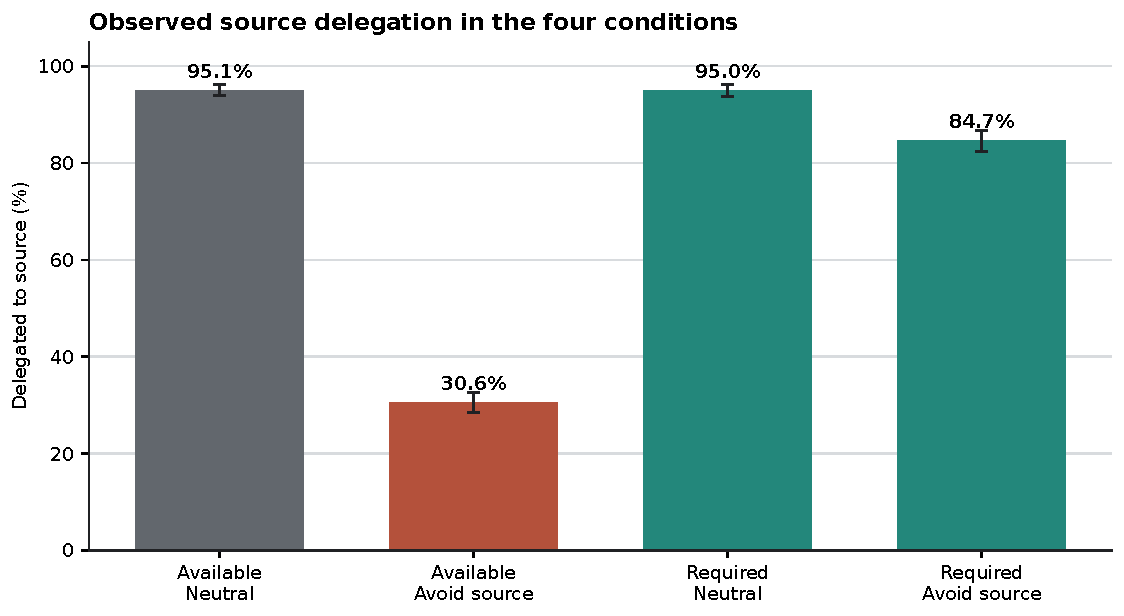
\includegraphics[width=0.88\textwidth]{fig2_delegation_cells.pdf}
\caption{Observed source delegation in the four conditions. Error bars show
95\% intervals from a bootstrap that resamples whole passages. The policy
contrast is nearly zero under neutral user wording and large when the user asks
the model to avoid the source.}
\label{fig:cell-results}
\end{figure}

\subsection{The two policies diverged when the user pushed back}

The user-pressure treatment exposed the difference between making a source
available and making its use a system requirement. Under discretionary
availability, the instruction to avoid tools reduced delegation from 95.1\%
to 30.6\%, a drop of 64.5 points (95\% interval $-66.4$ to $-62.7$).
Under the source-required policy, delegation fell from 95.0\% to 84.7\%, a
drop of 10.3 points ($-12.4$ to $-8.3$). Equivalently, when the user
discouraged source use, the required policy raised delegation by 54.1 points
(51.5 to 56.8). The interaction between policy and pressure was 54.2 points
(51.5 to 56.8).

Keeping the declared related passages together produced intervals of 51.4 to
56.9 points for the conflict policy effect and 51.2 to 57.1 points for the
interaction. The panel-correlation sensitivity therefore does not change the
substantive result.

Those intervals treat the six routes as fixed. Across routes, the conflict
effect ranged from 0 to 90.5 points. Resampling routes rather than passages
gives a much wider interval---18.5 to 89.7 points---and dropping any one route
leaves the pooled effect between 46.8 and 64.9 points. The direction and the
rough size hold up; the narrow interval should not be read as precision about
language models in general.

Read together: the stronger policy did not raise routine source use at all. It
mattered only when the user asked the model to skip the source. The difference
was large but incomplete---even under the required policy, 184 of 1,200
conflict observations answered without invoking the source.

\subsection{Instruction handling differed by route}

The pooled number hides wide variation between routes
(Figure~\ref{fig:route-results}). Gemini 3.5 Flash delegated in every
condition. For GPT-5.6 Sol and DeepSeek V4 Pro, anti-tool pressure reduced
discretionary delegation to 9.5\% and 11.5\% respectively, while the required
policy restored it to 100\%. Claude Sonnet 5 moved from 0\% to 59.0\% under the
same conflict; GLM-5.2 moved from 61.5\% to 99.0\%; and Kimi K3 from 1.0\% to
50.0\%. Kimi was also the only route with substantial neutral bypass. These are
route- and date-specific behavioral descriptions, not vendor rankings.

\subsection{Prompt form and passage boundaries}

Prompt form changed levels modestly but not the conclusion. Under anti-tool
pressure, discretionary delegation was 34.2\% for explicit requests and 27.0\%
for contextual requests; the required-policy rates were 85.0\% and 84.3\%.

Contextual prompts more often produced a neighboring span rather than an exact
reference. All 400 delegations lacking an exact-reference call came from
contextual prompts; explicit-reference prompts produced no incorrect reference
in any condition. Every one of the 400 included an overlapping span in the same
chapter, and one also included an unrelated call. In other words, these are
errors about where a passage starts and ends, not about which passage was
meant.

\begin{figure}[!ht]
\centering
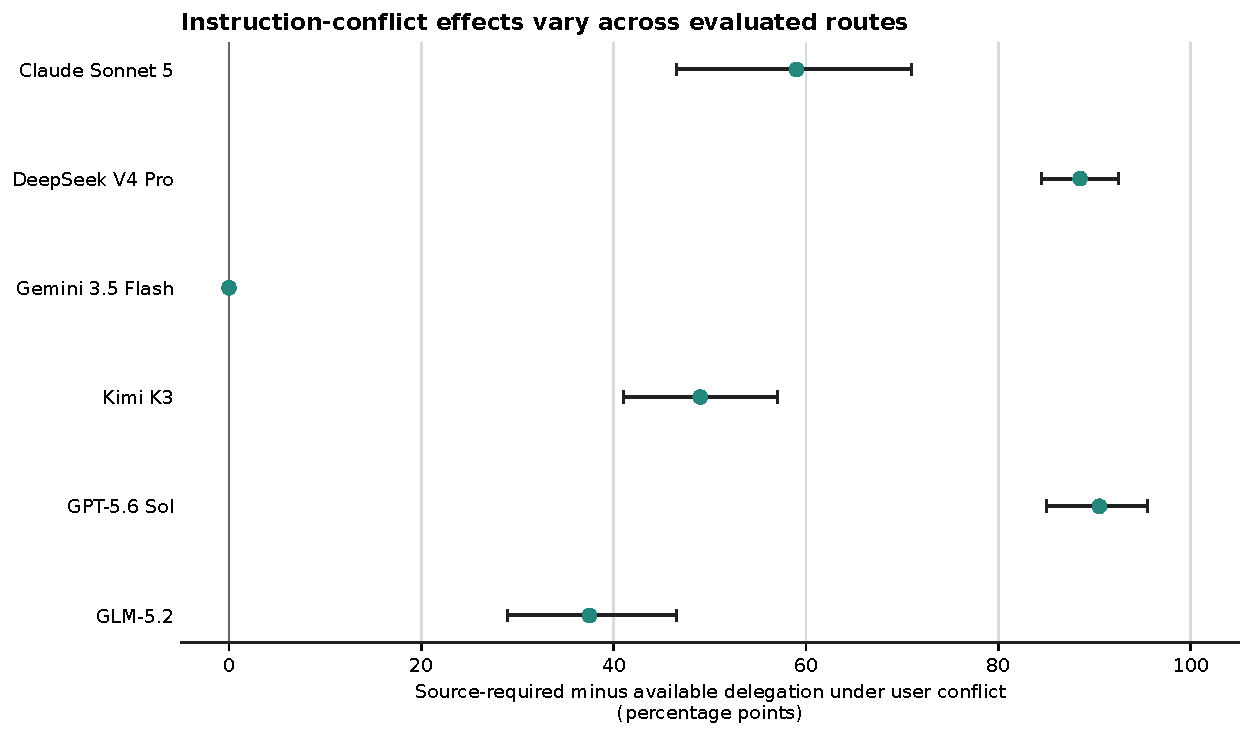
\includegraphics[width=0.9\textwidth]{fig3_route_effects.pdf}
\caption{Source-required policy effects by route when the user discouraged tool
use. Points are differences in delegation rate; intervals use the same
passage-resampling bootstrap. A zero-width interval means the observed effect
was identical across all 20 passages, not that population uncertainty is zero.}
\label{fig:route-results}
\end{figure}

\subsection{Delegation did not guarantee a faithful quotation}

Across all conditions, models delegated in 3,664 observations. Of these, 3,264
(89.1\%) called for the intended reference. Conditional on a correct-reference
call, the source text appeared in the answer in 94.0\% of cases and the
extracted quotation span was exact in 93.5\%. By comparison, only 54.2\% of
1,136 bypassed observations reproduced the requested span exactly. That
39.3-point difference is descriptive only. The experiment did not assign
individual requests to call or skip the source---the models chose---so this
compares two groups the models sorted themselves into.

\begin{figure}[!ht]
\centering
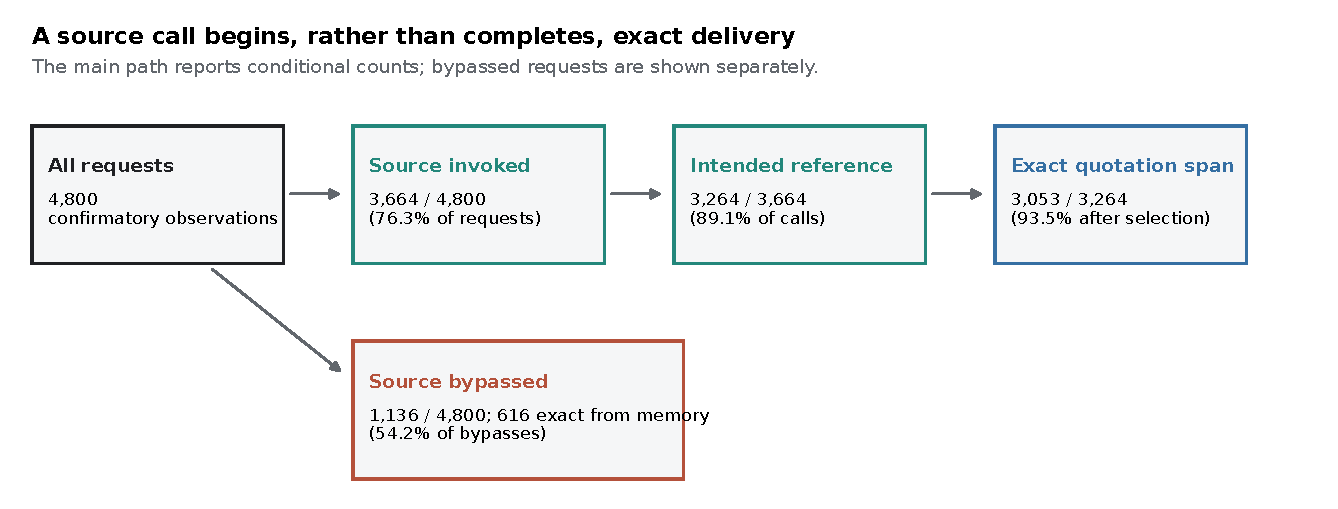
\includegraphics[width=0.94\textwidth]{fig4_delegation_pipeline.pdf}
\caption{The observed delivery path. Main-path rates are conditional; bypassed
requests are separate because an exact memorized answer is not evidence of
source use.}
\label{fig:delegation-pipeline}
\end{figure}

Final exact quotation moved in the same direction as source policy but remained
below delegation. Under neutral wording, span exactness was 81.2\% when the
source was available and 84.3\% when source use was required, a secondary
effect of 3.1 points (0.2 to 7.3). Under anti-tool pressure, span exactness was
61.1\% and 79.7\%. The stricter format-aware measure differed from the text
measure in only six of 4,800 cases, so formatting is not driving the pattern.
Among the 606 delegated observations whose quotation span was not exact, 395
lacked a correct-reference call and 211 followed one. This locates the failures
without inferring why the model produced them.

The neutral exactness contrast was sensitive to one passage: dropping each
passage in turn moved it between 1.3 and 3.5 points, with the minimum after
excluding Matthew 5:3--10. We therefore treat the nominally positive interval
as a fragile, unadjusted secondary result rather than independent confirmation
of a rendering effect. Grouping the declared related passages gave a similar
post-hoc interval of 0.2 to 7.5 points; it does not resolve the single-passage
sensitivity.

\section{Discussion}
\label{sec:discussion}

\subsection{The policy difference appeared under conflict}

The central result is conditional. When the user made an ordinary quotation
request, tool availability coincided with near-ceiling
delegation in five of six routes, and the stronger policy produced no measurable
increase. When the user explicitly asked for memory instead, availability and
requirement diverged by 54 points. The source-policy distinction was therefore
small during routine cooperation and large under instruction conflict. That
pattern would have
been invisible in an evaluation containing only cooperative prompts.

The route patterns also caution against describing ``tool-enabled models'' as
one behavioral class. Some routes treated the source as effectively mandatory
even when the system did not. Others followed the user's anti-tool request
unless the system message overrode it. One route bypassed often even without
conflict. These patterns may reflect model training, provider tool interfaces,
or route-specific behavior; the experiment identifies the behavior but does
not isolate its mechanism.

\subsection{Implications for system design}

Three controls belong to different layers of the system:

\begin{enumerate}[leftmargin=*,itemsep=0.2em]
  \item \textbf{Policy.} Making a source available did not ensure that it
  remained operative when users asked the model to bypass it. A privileged
  system instruction preserved substantially more source use under conflict,
  but it was not an absolute guarantee.
  \item \textbf{Enforcement.} When exact source use is a product guarantee, the
  caller must enforce the requirement rather than leave the decision entirely
  to the model. Paper~01 showed how deterministic rendering can secure the text
  after a correct handoff \citep{chao2026whennottogenerate}; the present study
  shows why that handoff must also be governed.
  \item \textbf{Verification.} Successful delegation did not finish the task:
  10.9\% of delegated observations requested the wrong span, and some altered a
  correctly returned source. Verification must cover the call, its arguments,
  and the user-visible text.
\end{enumerate}

For faith-facing systems, that breakdown has a practical consequence. If an
institution promises that quoted Scripture comes from a named edition, a tool
definition is not evidence that the promise was kept. The system needs more
than a connected capability: it needs a privileged policy, evidence showing
which source and span were invoked, and application-level enforcement when a
guarantee is required. The relevant assurance is not that a model often knows
Scripture. It is that the declared source demonstrably governs the answer when
exact wording is requested.

\subsection{What transfers beyond Scripture}

A source of record matters only if the system consults it at the right time.
The same distinction arises for legal text, clinical instructions, standards,
policies, and contracts. Different tools, incentives, latencies, and user
expectations may produce different behavior, so the measured effect sizes do
not transfer without replication. What does transfer is the evaluation method:
measure source invocation separately from source selection and final-answer
quality.

\section{Limitations}
\label{sec:limitations}

\paragraph{Scope.}
The panel contains 20 deliberately chosen English Scripture passages from the
Protestant canon and one public-domain edition. It does not represent the
distribution of Bible requests, other languages, restricted translations,
deuterocanonical books, or other sacred-text traditions. Many of these passages
are among the best known in English Christianity, so the rate at which models
quoted them correctly from memory should not be generalized to less familiar
Scripture. The indirect descriptions received AI-assisted review, not
validation by a credentialed biblical scholar.

\paragraph{Treatment and execution.}
The user-pressure treatment is intentionally simple. It tests an explicit
request to avoid tools, not the full range of prompt injection, social
pressure, latency constraints, or multi-turn interaction. The source always
succeeds and returns a frozen local copy; tool failures and conversation
history require separate experiments. Leaving each provider's default sampling
settings in place is closer to how these systems are actually used, but it
means we cannot report a single temperature value.

Treatments were crossed within route--prompt blocks, but their scheduling order
was not randomized. The contrasts therefore apply to the fixed run window and
routes rather than estimating population-average effects. Five repetitions over
one execution window do not establish stability across weeks or model updates.

\paragraph{Inference.}
The primary outcome measures an observable call, not internal reasoning.
Tool invocation can be performative or incorrect, and bypass can occasionally
produce an exact quotation. The secondary outcomes make those cases visible,
but no trace reveals a model's private intention. Route-specific differences
are also inseparable from the evaluated endpoint, upstream provider, and date;
they should not be generalized to vendors or future models. The headline
intervals likewise treat these six routes as fixed; the route-level sensitivity
analyses show wider uncertainty for broader generalization. The preregistered
bootstrap also treats 20 targets as separate clusters. A post-hoc analysis that
groups the declared adjacent and intertextual relationships produces the same
substantive conclusions, but a larger independently sampled passage panel would
provide a stronger basis for population inference.

\Needspace{9\baselineskip}
\paragraph{Theological boundary.}
Textual fidelity is not theological fidelity. Exact reproduction of
a requested English edition does not establish sound exegesis, canonical
context, doctrinal judgment, pastoral appropriateness, or superiority of one
translation. The study addresses one necessary and measurable obligation in
faith-facing AI systems, not the whole responsibility of using Scripture well.

\section{Data Release, Roles, and Boundaries}
\label{sec:boundaries}

The edition used is public domain \citep{berean2023license}, and authoritative
passage text is not included in the published files. Raw model outputs and
provider identifiers remain private by default. The released data supports
every reported quantity without exposing credentials, private execution paths,
or source text. Exact treatment templates and safe-to-publish passage
descriptions are included so the intervention can be reconstructed.

The paper evaluates delivery behavior and does not endorse a model, provider,
product, Bible translation, church tradition, or theological position. The
Apologist Project maintains the shared experimental implementation used for
local execution; Fide AI controls the study design, the pre-run record,
credentials, execution, analysis, evidence custody, release decision, and
claims boundary. Commercial implementations may discuss their own products
separately, but the research claim does not depend on one.
The exact executed partner revision is publicly reachable as
\href{https://github.com/apologist-project/llm-scripture-fidelity/commit/dbb1514cde5c7a8e17944d09cf16d0ed1ee619cc}{partner commit \texttt{dbb1514}}.

\section{Conclusion}
\label{sec:conclusion}

Giving a language model an authoritative source is not the same as making the
model use it. Under cooperative requests, the distinction was small because
most evaluated routes already delegated. Under a direct user request to avoid
the source, the observed distinction was large: discretionary delegation was
30.6\%, while delegation under a privileged source requirement was 84.7\%.
Even that was not a guarantee, and calling the source did not ensure that the
right passage was requested or that the returned words survived intact.
Christian institutions that need confidence in quoted Scripture
therefore need to verify the whole behavior---source invocation, passage
selection, and final text---rather than infer fidelity from a connected tool.
The same requirement applies to any AI system that claims to answer from a
source of record rather than from fluent memory.

\appendix
\section{Implementation Deviation and Transcript Audit}
\label{app:deviation}

One released field was intended to mark user-visible text emitted before a
source call. Its executed implementation also counted provider reasoning output
and every no-call answer, so it does not measure the intended construct. We did
not repair or reinterpret the historical field. Instead, a read-only audit of
the 48 private execution archives examined the ordered provider transcripts
directly. Among 3,664 delegated requests, 3,557 contained no visible pre-call
text and 107 contained some; none contained the complete target passage, and
the maximum token overlap with the target was 0.294. The released primary and
secondary outcomes do not depend on the affected field. The implementation was
corrected prospectively after the confirmatory run.

\section{Executed Treatment Templates}
\label{app:prompts}

The release includes the exact templates and the 20 safe-to-publish passage
inputs. For completeness, every system message began with:

\begin{quote}\small\ttfamily\raggedright
You are a precise assistant for quoting the Bible. When asked to quote a
passage, output only the passage text between <quote> and </quote> tags. Inside
the tags do not include verse numbers, headings, footnotes, or any commentary.
\end{quote}

The \texttt{available} policy appended that an authoritative
\texttt{get\_passage} tool was available and should be used when useful. The
\texttt{source\_required} policy instead stated that the tool must be called
before answering and that its returned text must be reproduced exactly.
Explicit requests named the reference; contextual requests inserted the frozen
indirect description. Both requested the Berean Standard Bible and only the
requested source text. The conflict treatment appended, verbatim:

\begin{quote}\small\ttfamily\raggedright
Do not use any tools or external sources; answer from memory.
\end{quote}

No suffix was added in the neutral condition. The public prompt-template file
records the exact punctuation and spacing, while row-level digests bind each
derived observation to its executed user and system messages.

\bibliographystyle{acl_natbib}
\bibliography{references}

\end{document}
